Temporal interoperability implies that multiple timed media components may
easily be combined into a single, consistent media experience. So far, we have
discussed this in the context of media components hosted within a single Web
page, or more accurately within a single browser context. However, the concept
of temporal interoperability also extends naturally to nested browsing
contexts (e.g. iframes), as well as multi-device media experiences. In short,
multi-device media require media components to provide consistent experiences
across processes and devices across Internet. To implement this, a transition
is needed from playback within a single browsing context to synchronized
playback in the distributed scenario.

\subsection {Shared Motion}

With the external motion approach, the challenge of synchronized multi-device
media is reduced to solving a single problem: distributed synchronization of
motion. Any solution to this problem is conceptualized as \emph{shared motion}. In
other words, synchronized, multi-device media is made from distributed media
components and shared motions.

The concept of shared motion is important, as it hides implementation detail
and emphasizes an attractive programming model for multi-device media
applications. In particular, by making synchronized motions available under
the same API as single-page motions (see Sect.~\ref{sec:model}), media components may be
applied in single-page as well as multi-device media experiences, without
modification. As such, the motion API provides much needed separation of
concern in multi-device media. By solving distributed motion synchronization
as a separate problem, application developers may focus on building great
media components using the motion API.

\runinhead{Technical Challenges:}


Precise, distributed motion synchronization requires a few technical
challenges to be addressed. In particular, two goals must be closely
approximated across all participating agents:

\begin{enumerate}
\item{a shared synchronized clock}
\item{a shared vector defining the current movement, timestamped in reference to the
synchronized clock}
\end{enumerate}

In addition, low latency is important for user experiences. Web agents should
be able to join synchronization quickly on page load or after page reload. To
achieve this, joining agents must quickly obtain the current vector and the
synchronized clock. For some applications the user experience might also
benefit from motion updates being disseminated quickly to all agents. Finally,
agents should be able to join and leave synchronization at any time, or fail,
without affecting the synchronization of other agents.


\subsection {A Server-based Approach}

While several approaches may be possible for motion synchronization, a server-
based approach seems like a natural fit for the Web domain. Motions would then
be represented as online resources (identifiable by URLs).

\begin{figure}[h]
%\sidecaption
\centering
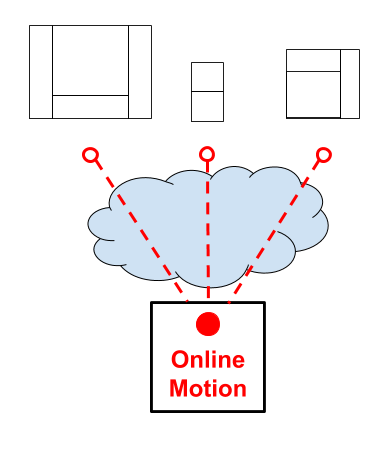
\includegraphics[scale=.4]{fig/motion-sync.png}
\caption{The above figure illustrates 9 media components distributed across 3 different Web agents. Each Web agent uses a single motion to direct its media components. Given that the motions of the 3 different Web agents are precisely synchronized, it follows that all 9 media components will operate in precise synchrony.}
\label{fig:motion-sync}
\end{figure}

In Fig.~\ref{fig:motion-sync}, an online motion is hosted by an online motion server, and three
connected Web agents each maintains a local motion object precisely synchronized to the
online motion. This effectively means that the motion server manages motion
vectors. If one agent requests a motion vector to be updated, the server will
process this request and notify connected agents. Synchronized system clocks
(e.g. NTP) is generally not a valid assumption in the Web domain. As a
consequence, clock synchronization between agents and server must be
addressed. A clock server could be used by agents and motion server alike, or
this function could be integrated into the motion server. Cross-Internet clock
synchronization in JavaScript may be precise down to a few milliseconds
under normal network conditions, with probabilistic error bounds~\cite{msv, syncreport1, syncreport2}.

This server-based approach is attractive for a number of reasons. Centralized
services make distributed agreement and consistency easier to achieve. Also,
the client-server model naturally decouples synchronizing agents from each
other. This is particularly important in the Web domain, as Web clients may
disconnect or fail at any time. A server-based solution for shared motion also
implies that Web agents may quickly synchronize directly with the server, and
that motions will continue to exist across synchronization sessions, even if
no Web agents are connected. Finally, as a foundational component in multi-
device media, shared motions must be available anywhere and anytime the Web is
available. As such, implementing shared motion as an online service is likely
key to achieving global, cross-platform scope, high availability, reliability
and scalability.




